\begin{figure}[H]
    \centering
    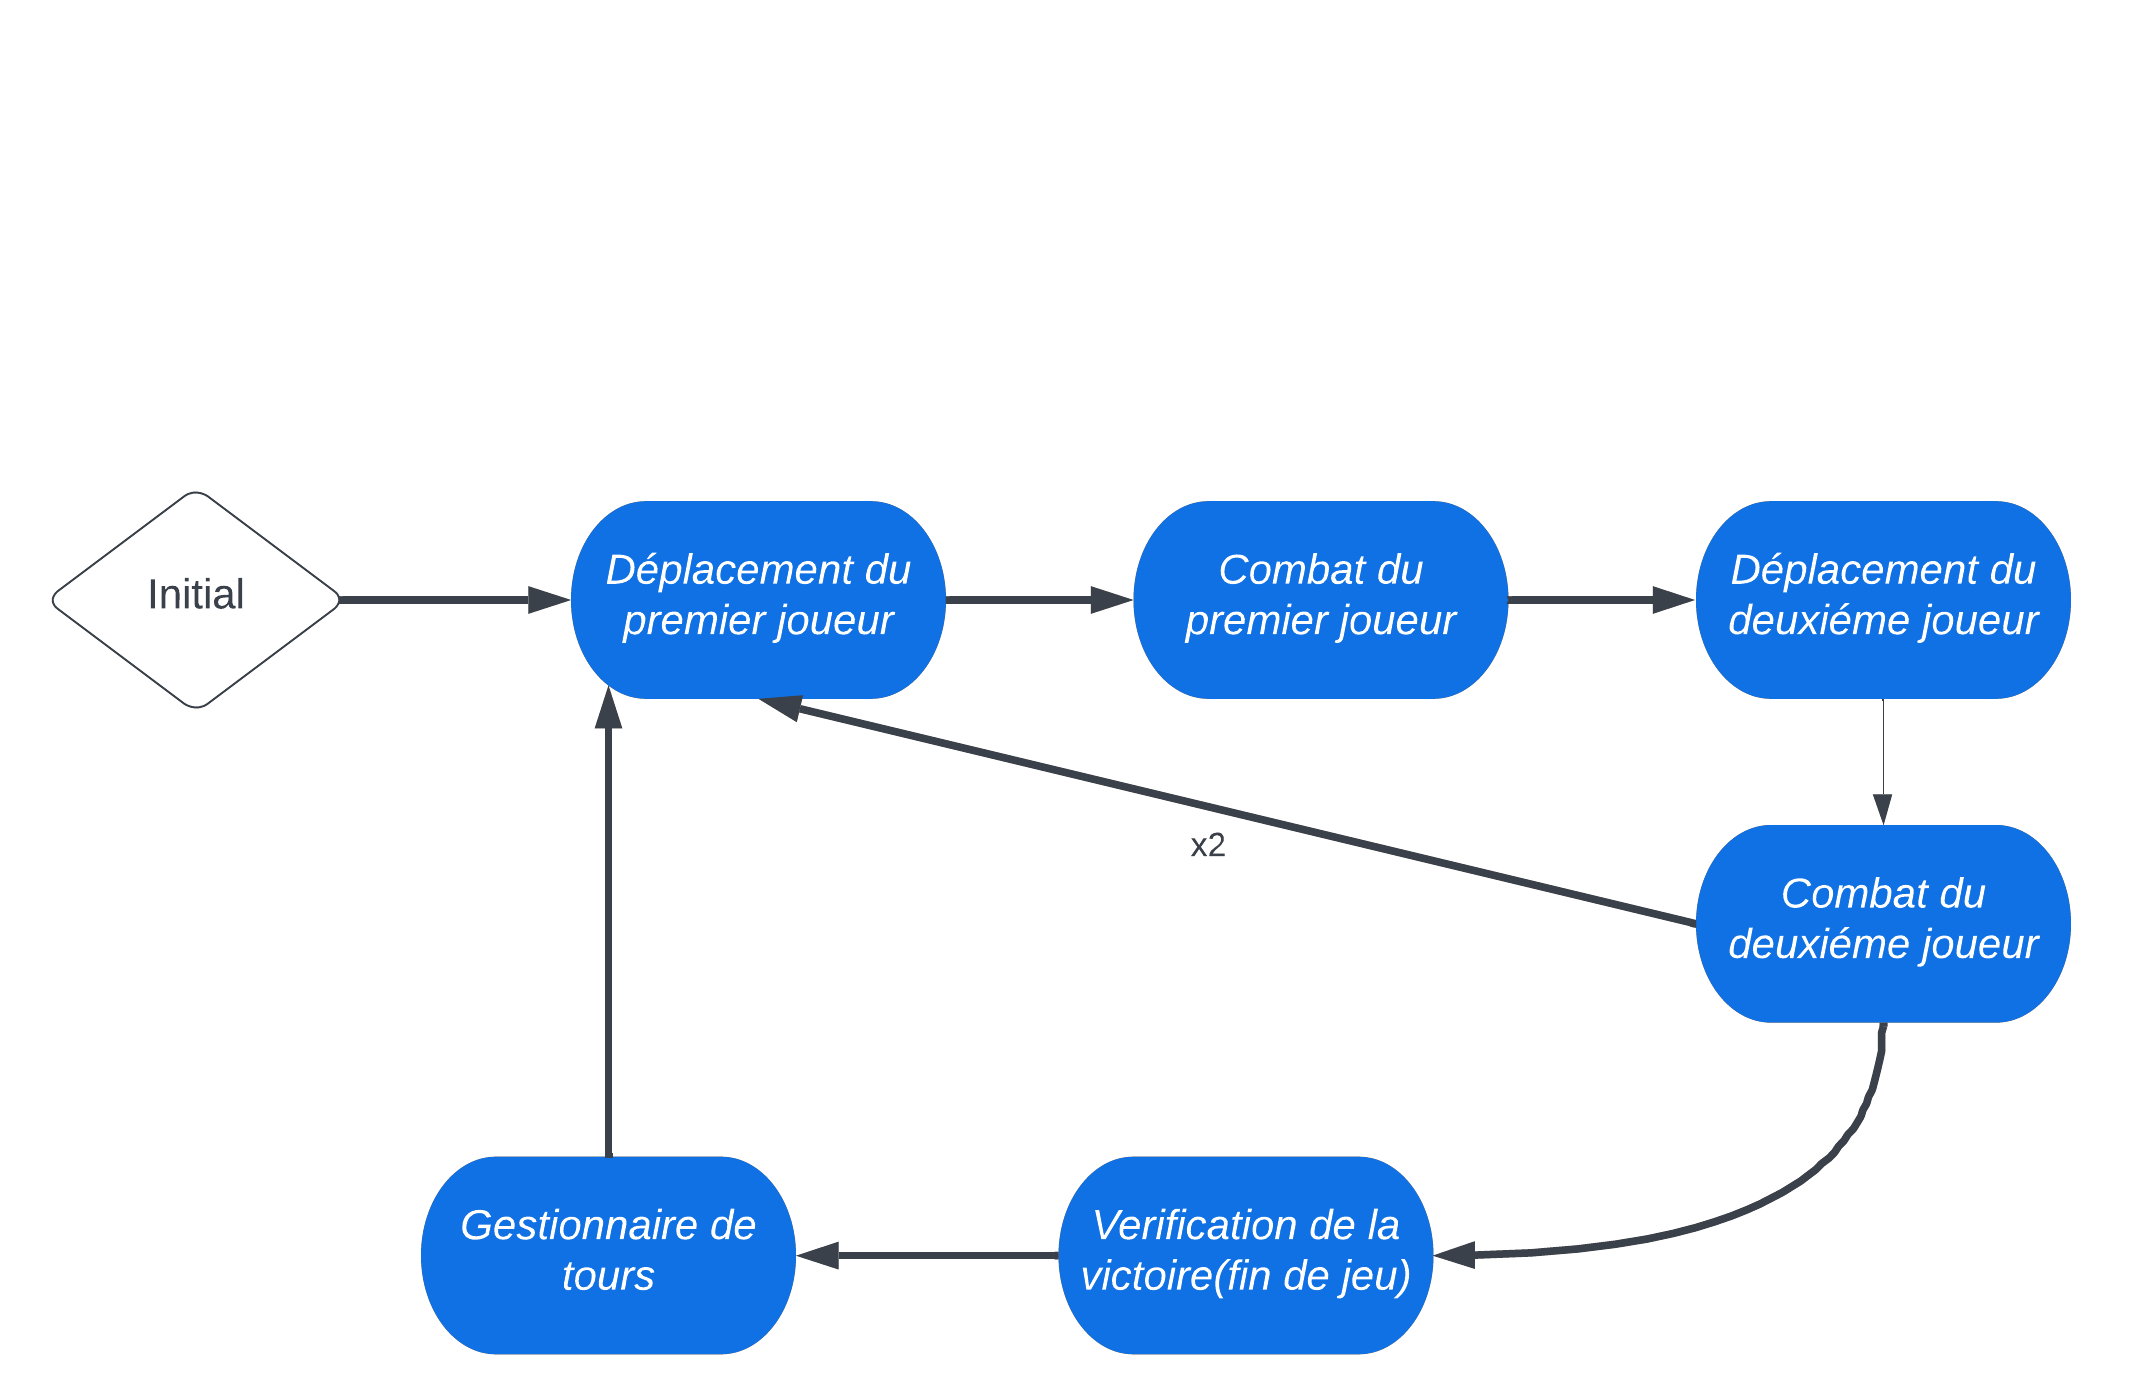
\includegraphics[scale=0.2]{data/State_Machine.png}
    \caption{Schéma de la machine d'état implémentée}
    \label{fig:schema_state_machine}
\end{figure}

Le schéma de l'automate dans la figure ci-dessus est une version simplifiée de notre automate, car, comme vous pouvez le voir, elle contient une transition x2, qui signifie la répétition des 4 premières phases une autre fois pour chaque tour, ce qui est exigée dans les règles.

Nous avons décidé de supprimer plusieurs phases à cause du manque du temps. Ces phases sont : la phase des événements spéciaux, car elle était très compliquée à implémenter, la phase de la supériorité aérienne, car nous n'avons pas implémenté les unités aériennes, la phase de renforts, car nous n'avons pas eu le temps d'implémenter une tactique de renfort, la phase d'allocation, car nous avons fait en sorte que les joueurs ont qu'une seule base, et cette phase servait principalement pour l'activation de plusieurs bases, la phase d'initiative, car nous avons fait en sorte que l'ordre de jeu ne change pas entre tours et finalement la phase de supply attrition, car nous faisons déjà ce qu'elle est censée faire a chaque début de phase de mouvement.

Cela laisse finalement 10 phases en total, dont la phase de mouvement du premier joueur, la phase de combat du premier joueur, le phase de mouvement du deuxième joueur et la phase de combat du deuxième joueur se répètent 2 fois, car c'est exigé que dans un tour il faut qu'un joueur puisse bouger ses unités et attaquer deux fois. Ensuite nous avons la phase de vérification de fin de jeu(ou de la victoire), qui vérifie si le nombre de tours dépasse 38, dans ce cas le premier joueur gagne, ou si un des joueurs a perdu toutes ses unités, et dans ce cas, le joueur avec des unités restantes gagne. La dernière phase est la phase du gestionnaire de tours, qui met simplement à jour le nombre de tours en augmentant par 1 le nombre du tour actuel.

Nous utilisons cette machine d'état pour gérer toutes les commandes du jeu, pour vérifier les approvisionnements des unités, pour savoir si le joueur peut effectuer une action dans cette phase, etc. Nous avons donc une machine d'état qui permet de gérer essentiellement tout le jeu, vu que ce dernier dépend complètement de cette machine d'état.